%package list
\documentclass{article}
\usepackage[top=3cm, bottom=3cm, outer=3cm, inner=3cm]{geometry}
\usepackage{multicol}
\usepackage{graphicx}
\usepackage{url}
%\usepackage{cite}
\usepackage{hyperref}
\usepackage{array}
%\usepackage{multicol}
\newcolumntype{x}[1]{>{\centering\arraybackslash\hspace{0pt}}p{#1}}
\usepackage{natbib}
\usepackage{pdfpages}
\usepackage{multirow}
\usepackage[normalem]{ulem}
\useunder{\uline}{\ul}{}
\usepackage{svg}
\usepackage{xcolor}
\usepackage{listings}

\lstdefinestyle{ascii-tree}{
    literate={├}{|}1 {─}{--}1 {└}{+}1 
  }
\lstset{basicstyle=\ttfamily,
  showstringspaces=false,
  commentstyle=\color{red},
  keywordstyle=\color{blue}
}
%\usepackage{booktabs}
\usepackage{caption}
\usepackage{subcaption}
\usepackage{float}
\usepackage{array}

\newcolumntype{M}[1]{>{\centering\arraybackslash}m{#1}}
\newcolumntype{N}{@{}m{0pt}@{}}


%%%%%%%%%%%%%%%%%%%%%%%%%%%%%%%%%%%%%%%%%%%%%%%%%%%%%%%%%%%%%%%%%%%%%%%%%%%%
%%%%%%%%%%%%%%%%%%%%%%%%%%%%%%%%%%%%%%%%%%%%%%%%%%%%%%%%%%%%%%%%%%%%%%%%%%%%
\newcommand{\itemEmail}{kllacma@unsa.edu.pe}
\newcommand{\itemStudent}{Kevin Andree Llacma Quispe}
\newcommand{\itemCourse}{Programacion web 2}
\newcommand{\itemCourseCode}{20200585}
\newcommand{\itemSemester}{I}
\newcommand{\itemUniversity}{Universidad Nacional de San Agustín de Arequipa}
\newcommand{\itemFaculty}{Facultad de Ingeniería de Producción y Servicios}
\newcommand{\itemDepartment}{Departamento Académico de Ingeniería de Sistemas e Informática}
\newcommand{\itemSchool}{Escuela Profesional de Ingeniería de Sistemas}
\newcommand{\itemAcademic}{2024 - A}
\newcommand{\itemInput}{-}
\newcommand{\itemOutput}{-}
\newcommand{\itemPracticeNumber}{03}
\newcommand{\itemTheme}{Javascript}
%%%%%%%%%%%%%%%%%%%%%%%%%%%%%%%%%%%%%%%%%%%%%%%%%%%%%%%%%%%%%%%%%%%%%%%%%%%%
%%%%%%%%%%%%%%%%%%%%%%%%%%%%%%%%%%%%%%%%%%%%%%%%%%%%%%%%%%%%%%%%%%%%%%%%%%%%

\usepackage[english,spanish]{babel}
\usepackage[utf8]{inputenc}
\AtBeginDocument{\selectlanguage{spanish}}
\renewcommand{\figurename}{Figura}
\renewcommand{\refname}{Referencias}
\renewcommand{\tablename}{Tabla} %esto no funciona cuando se usa babel
\AtBeginDocument{%
	\renewcommand\tablename{Tabla}
}

\usepackage{fancyhdr}
\pagestyle{fancy}
\fancyhf{}
\setlength{\headheight}{30pt}
\renewcommand{\headrulewidth}{1pt}
\renewcommand{\footrulewidth}{1pt}
\fancyhead[L]{\raisebox{-0.2\height}{
\includegraphics[width=3cm]{img/logo_episunsa.png}}}
\fancyhead[C]{\fontsize{7}{7}\selectfont	\itemUniversity \\ \itemFaculty \\ \itemDepartment \\ \itemSchool \\ \textbf{\itemCourse}}
\fancyhead[R]{\raisebox{-0.2\height}{
\includegraphics[width=1.2cm]{img/logo_abet}}}
\fancyfoot[L]{Estudiante Kevin Llacma}
\fancyfoot[C]{\itemCourse}
\fancyfoot[R]{Página \thepage}

% para el codigo fuente

\usepackage{listings}
\usepackage{color, colortbl}
\definecolor{dkgreen}{rgb}{0,0.6,0}
\definecolor{gray}{rgb}{0.5,0.5,0.5}
\definecolor{mauve}{rgb}{0.58,0,0.82}
\definecolor{codebackground}{rgb}{0.95, 0.95, 0.92}
\definecolor{tablebackground}{rgb}{0.8, 0, 0}

\lstset{frame=tb,
	language=bash,
	aboveskip=3mm,
	belowskip=3mm,
	showstringspaces=false,
	columns=flexible,
	basicstyle={\small\ttfamily},
	numbers=none,
	numberstyle=\tiny\color{gray},
	keywordstyle=\color{blue},
	commentstyle=\color{dkgreen},
	stringstyle=\color{mauve},
	breaklines=true,
	breakatwhitespace=true,
	tabsize=3,
	backgroundcolor= \color{codebackground},
}

\begin{document}
	
	\vspace*{10px}
	
	\begin{center}	
		\fontsize{17}{17} \textbf{ Informe de Laboratorio \itemPracticeNumber}
	\end{center}
	\centerline{\textbf{\Large Tema: \itemTheme}}
	%\vspace*{0.5cm}	

	\begin{flushright}
		\begin{tabular}{|M{2.5cm}|N|}
			\hline 
			\rowcolor{tablebackground}
			\color{white} \textbf{Nota}  \\
			\hline 
			     \\[30pt]
			\hline 			
		\end{tabular}
	\end{flushright}	

	\begin{table}[H]
		\begin{tabular}{|x{4.7cm}|x{4.8cm}|x{4.8cm}|}
			\hline 
			\rowcolor{tablebackground}
			\color{white} \textbf{Estudiante} & \color{white}\textbf{Escuela}  & \color{white}\textbf{Asignatura}   \\
			\hline 
			{\itemStudent \par \itemEmail} & \itemSchool & {\itemCourse \par Semestre: \itemSemester \par Código: \itemCourseCode}     \\
			\hline 			
		\end{tabular}
	\end{table}		
	
	\begin{table}[H]
		\begin{tabular}{|x{4.7cm}|x{4.8cm}|x{4.8cm}|}
			\hline 
			\rowcolor{tablebackground}
			\color{white}\textbf{Laboratorio} & \color{white}\textbf{Tema}  & \color{white}\textbf{Duración}   \\
			\hline 
			\itemPracticeNumber & \itemTheme & 04 horas   \\
			\hline 
		\end{tabular}
	\end{table}
	
	\begin{table}[H]
		\begin{tabular}{|x{4.7cm}|x{4.8cm}|x{4.8cm}|}
			\hline 
			\rowcolor{tablebackground}
			\color{white}\textbf{Semestre académico} & \color{white}\textbf{Fecha de inicio}  & \color{white}\textbf{Fecha de entrega}   \\
			\hline 
			\itemAcademic & \itemInput &  \itemOutput  \\
			\hline 
		\end{tabular}
	\end{table}
\title{Programación Web\\Laboratorio 03\\Tema: JavaScript}

\maketitle


\section{Marco teórico}

\subsection{Vim}
Vim es un editor de texto altamente configurable creado para hacer que la creación y el cambio de cualquier tipo de texto sean muy eficientes. Se incluye como "viçon la mayoría de los sistemas UNIX y con Apple OS X.

Vim es muy estable y se desarrolla continuamente para mejorar aún más. Entre sus características se encuentran:
\begin{itemize}
    \item árbol de deshacer persistente de varios niveles
    \item amplio sistema de complementos
    \item soporte para cientos de lenguajes de programación y formatos de archivo
    \item poderosa búsqueda y reemplazo
    \item se integra con muchas herramientas
\end{itemize}


\begin{lstlisting}[language=bash]
$ sudo apt-get install vim  # Vim en GNU/Linux
$ brew install macvim  # Vim en MacOSX
\end{lstlisting}

\subsection{Visual Studio Code}
Visual Studio Code es un editor de código fuente ligero pero potente que se ejecuta en su escritorio y está disponible para Windows, macOS y Linux. Viene con soporte integrado para JavaScript, TypeScript y Node.js y tiene un rico ecosistema de extensiones para otros lenguajes y tiempos de ejecución (como C++, C, Java, Python, PHP, Go, .NET).

Videotutoriales: \url{https://code.visualstudio.com/docs/getstarted/introvideos}

Descarga: \url{https://code.visualstudio.com/Download}


\section{Desarollo del lab}
\subsection{Ejercicio 1}
\textbf{Cree un teclado random para banca por internet. }
\\Para este ejericio de uso un html basico que se dio. Se agrego style para los botones de los numeros.

\\.teclado-container: Configura el contenedor del teclado para usar un diseño de cuadrícula de 3 columna.
\\.tecla: Estiliza cada tecla del teclado.
\\.input-display: Estiliza el campo de entrada donde se muestran los números seleccionados.



    \begin{figure}[H]
		          \centering
		          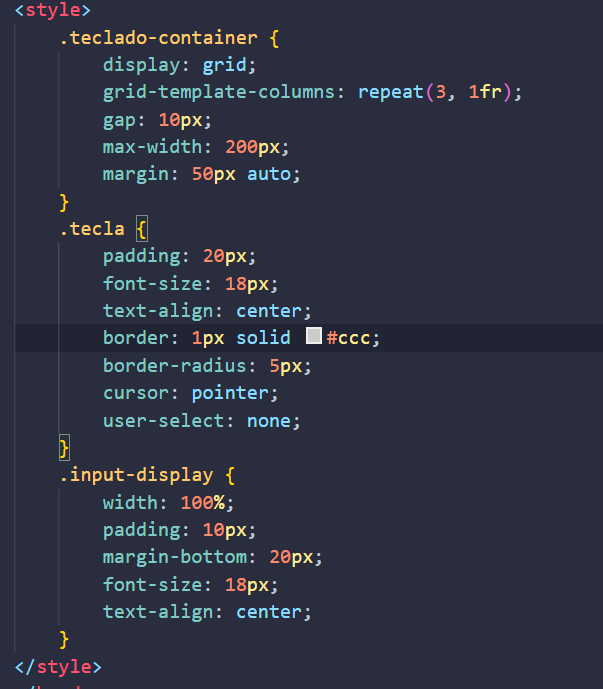
\includegraphics[width=0.8\textwidth,keepaspectratio]                       {img/styleTeclado.png}
		             %\includesvg{img/automata.svg}
		              %\label{img:mot2}
		              %\caption{Product backlog.}
    \end{figure}
\\
\\\textbf{-<div id="teclado-container"></div>:} Un contenedor para las teclas del teclado numérico.
\\\textbf{-<input type="text" id="input-display" class="input-display" readonly>:} Un campo de entrada que muestra los números seleccionados, es de solo lectura.
\\\textbf{-<script src="teclado.js"></script>:} Incluye el archivo JavaScript que contiene la lógica del teclado.
    \begin{figure}[H]
		          \centering
		          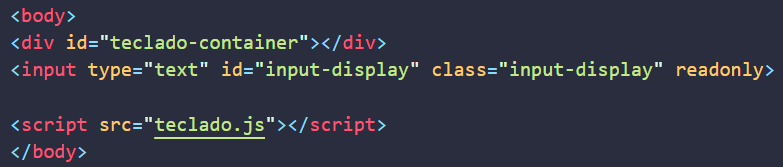
\includegraphics[width=0.8\textwidth,keepaspectratio]                       {img/bodyTeclado.png}
		             %\includesvg{img/automata.svg}
		              %\label{img:mot2}
		              %\caption{Product backlog.}
    \end{figure}
\\
\\Ahora en javaScript tenemos

\\\textbf{document.addEventListener('DOMContentLoaded', function() ):} Asegura que el código JavaScript se ejecute solo después de que todo el contenido HTML haya sido completamente cargado.

\\\textbf{const tecladoContainer = document.getElementById('teclado-container'):} Selecciona el contenedor donde se crearán las teclas.
\\\textbf{const inputDisplay = document.getElementById('input-display'):} Selecciona el campo de entrada donde se mostrarán los números seleccionados.

\\\textbf{const numeros = Array.from({ length: 10 }, (_, i) => i):} Crea un arreglo con los números del 0 al 9.


     \begin{figure}[H]
		          \centering
		          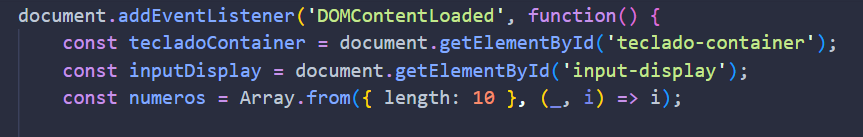
\includegraphics[width=0.8\textwidth,keepaspectratio]                       {img/eventoTeclado.png}
		             %\includesvg{img/automata.svg}
		              %\label{img:mot2}
		              %\caption{Product backlog.}
    \end{figure}
\\
\\Función barajar:
\\Esta función toma un arreglo y lo baraja usando el algoritmo de Fisher-Yates.
function barajar(array) { ... }: Recibe un arreglo y lo baraja aleatoriamente.
    \begin{figure}[H]
		          \centering
		          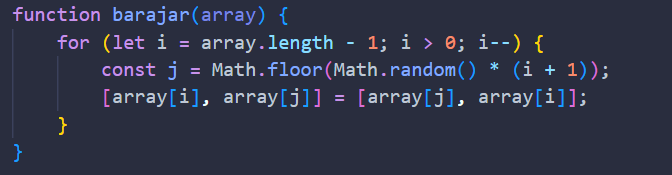
\includegraphics[width=0.8\textwidth,keepaspectratio]                       {img/barajarTeclado.png}
		             %\includesvg{img/automata.svg}
		              %\label{img:mot2}
		              %\caption{Product backlog.}
    \end{figure}
\\
\\Función crearTeclado:
\\Llama a barajar(numeros) para mezclar los números.
\\Limpia el contenedor del teclado con tecladoContainer.innerHTML = '';.
\\Para cada número en el arreglo barajado:
\begin{itemize}
    \item Crea un nuevo elemento div para representar una tecla.
    \item Asigna la clase tecla al div.
    \item Establece el contenido de texto del div al número actual.
    \item Agrega un evento click al div para que, cuando se haga clic, el número se agregue al valor del inputDisplay.
    \item Añade el div al contenedor del teclado.
\end{itemize}
    \begin{figure}[H]
		          \centering
		          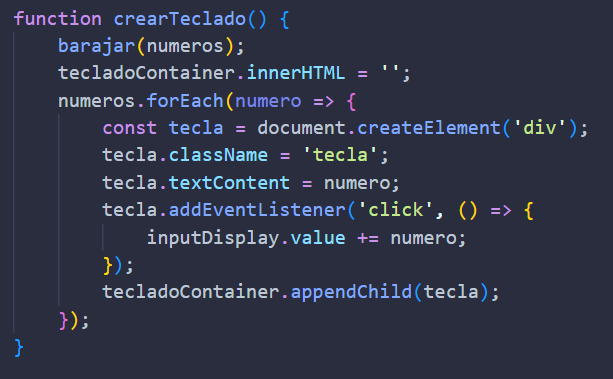
\includegraphics[width=0.8\textwidth,keepaspectratio]                       {img/crearTeclado.png}
		             %\includesvg{img/automata.svg}
		              %\label{img:mot2}
		              %\caption{Product backlog.}
    \end{figure}
\\
\\Finalmente se inicializa

    \begin{figure}[H]
		          \centering
		          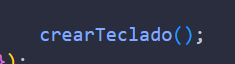
\includegraphics[width=0.8\textwidth,keepaspectratio]                       {img/iniciaTeclado.png}
		             %\includesvg{img/automata.svg}
		              %\label{img:mot2}
		              %\caption{Product backlog.}
    \end{figure}

\\
\\Algunas pruebas de la aleatoriedad de los numeros y el campo se encuentra abajo

    \begin{figure}[H]
		          \centering
		          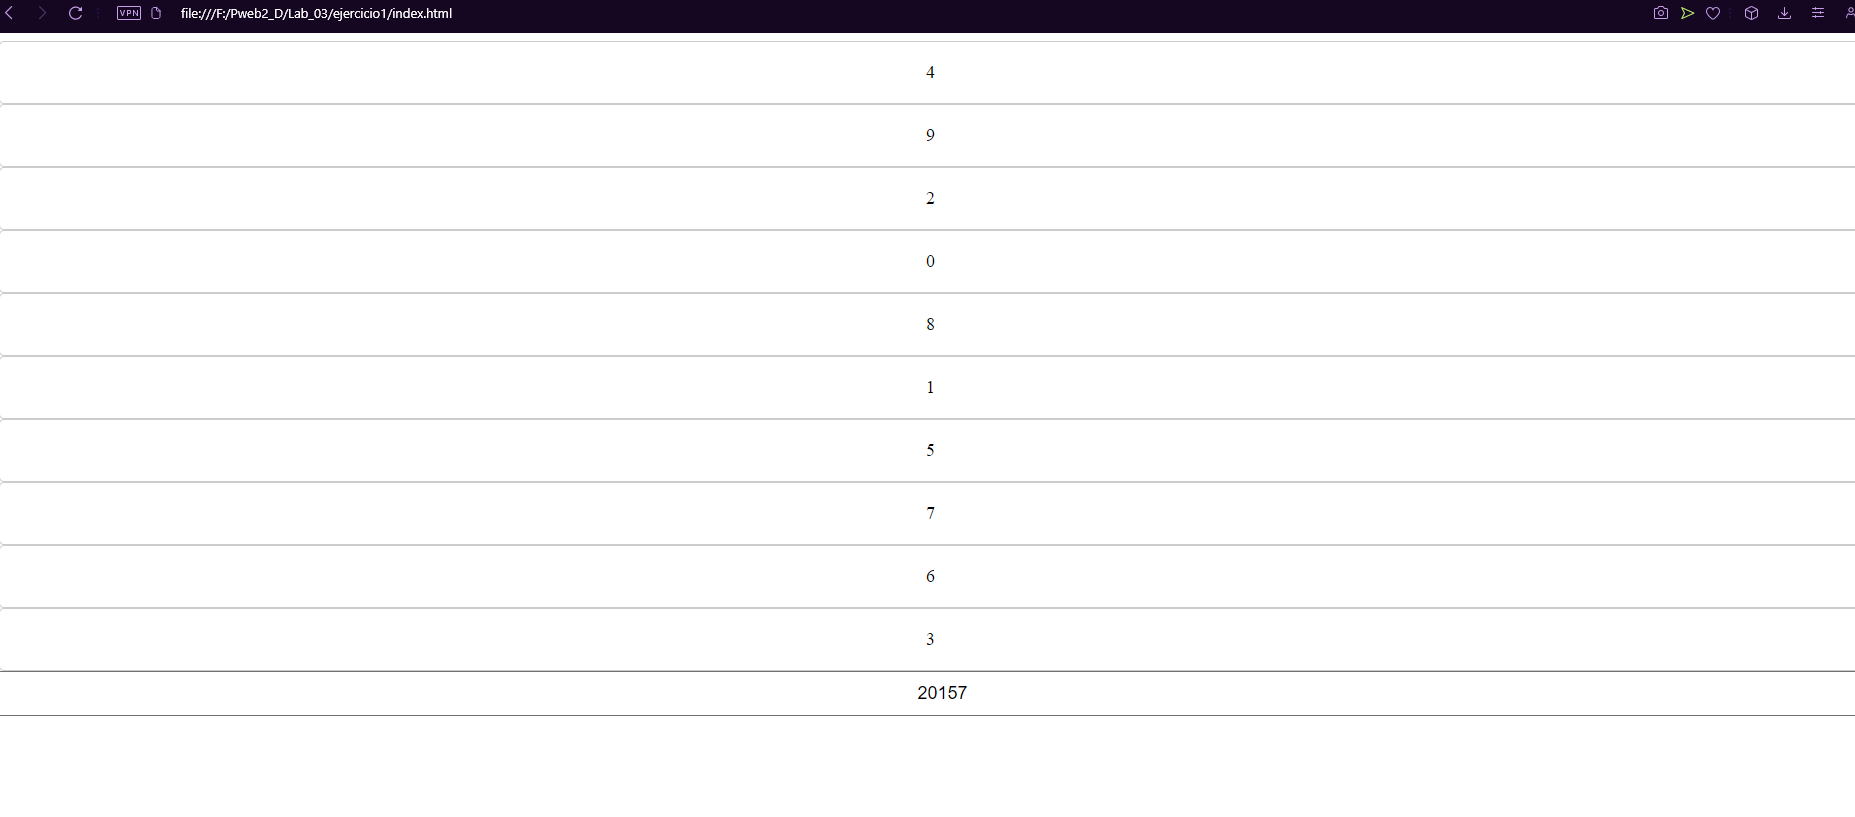
\includegraphics[width=0.8\textwidth,keepaspectratio]                       {img/pruebaTeclado1.png}
		             %\includesvg{img/automata.svg}
		              %\label{img:mot2}
		              %\caption{Product backlog.}
    \end{figure}    
\\
\\
     \begin{figure}[H]
		          \centering
		          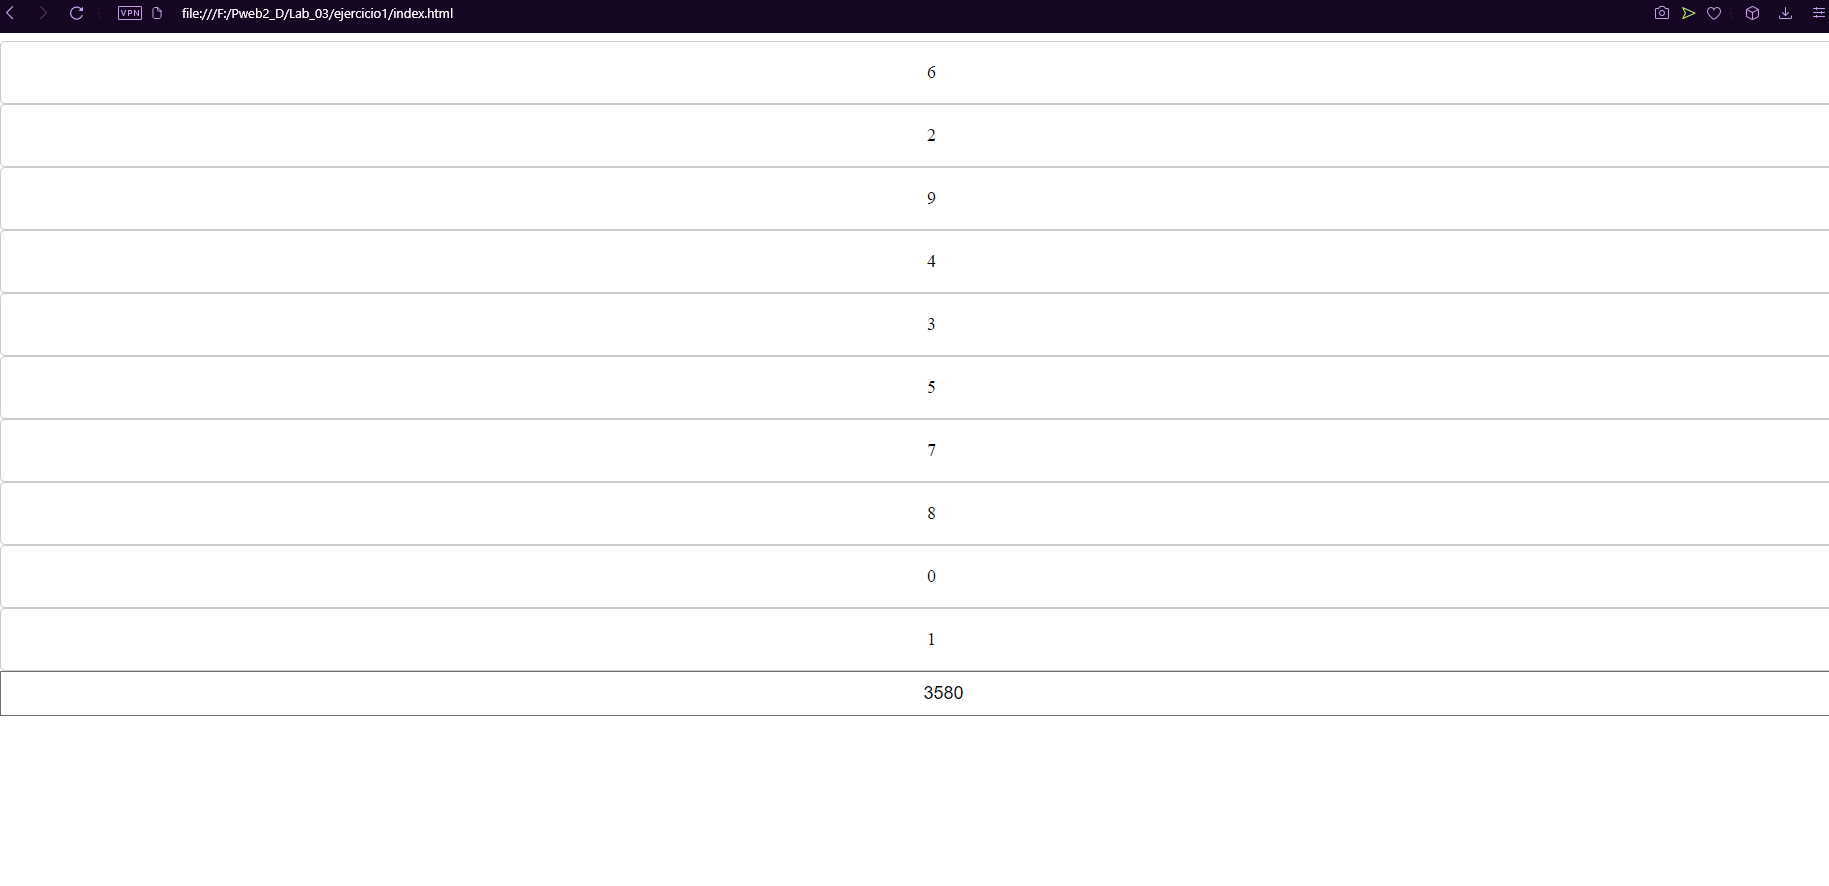
\includegraphics[width=0.8\textwidth,keepaspectratio]                       {img/pruebaTeclado2.png}
		             %\includesvg{img/automata.svg}
		              %\label{img:mot2}
		              %\caption{Product backlog.}
    \end{figure}    
\subsection{Ejercicio 2}
\\Para este ejercicio se uso el mismo formato del anterior ejercicio (un html basico con styles) y su logica javascript
\\En el body tenemos los botones de la calculadora
\\\textbf{-<div class="calculadora">:} Contenedor de la calculadora que incluye los botones y la pantalla.
\\\textbf{-<div id="pila-operaciones" class="pila-operaciones"></div>:} Contenedor para mostrar el historial de operaciones.
\\\textbf{-<script src="calculadora.js"></script>:} Archivo JavaScript que contiene la lógica.

     \begin{figure}[H]
		          \centering
		          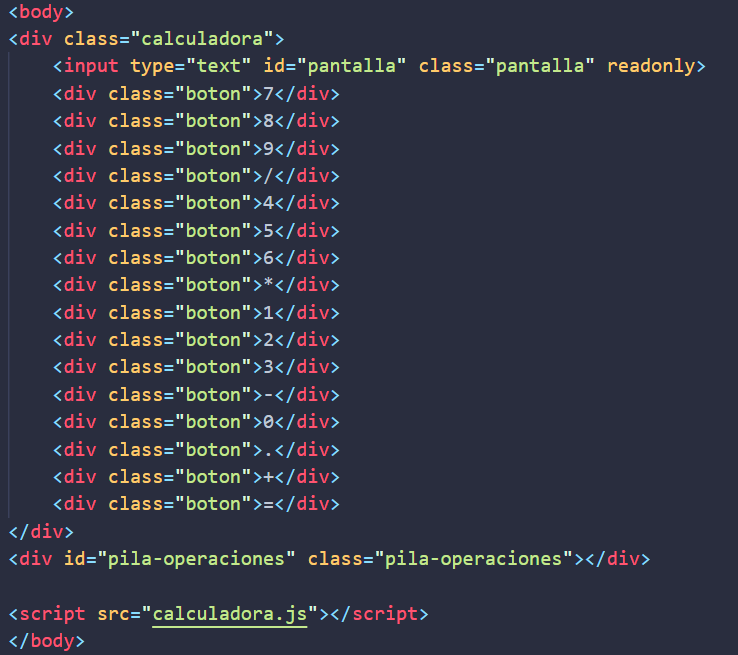
\includegraphics[width=0.8\textwidth,keepaspectratio]                       {img/bodyCal.png}
		             %\includesvg{img/automata.svg}
		              %\label{img:mot2}
		              %\caption{Product backlog.}
    \end{figure}  
\\
\\Para la logica del ejercicio tenemos :
\\\textbf{const pantalla = document.getElementById('pantalla'):} Selecciona el campo de entrada donde se mostrarán las expresiones y resultados.
\\\textbf{const botones = document.querySelectorAll('.boton'):} Selecciona todos los botones de la calculadora.
\\\textbf{const pilaOperaciones = document.getElementById('pila-operaciones'):} Selecciona el contenedor donde se mostrará el historial de operaciones.

 \begin{figure}[H]
		          \centering
		          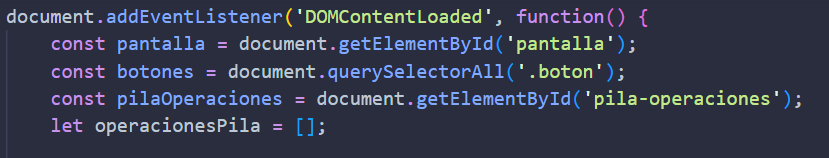
\includegraphics[width=0.8\textwidth,keepaspectratio]                       {img/DOMCal.png}
		             %\includesvg{img/automata.svg}
		              %\label{img:mot2}
		              %\caption{Product backlog.}
    \end{figure}  
\\
\\Evnetos de clic a los botnes
\\botones.forEach(boton => { ... });: Itera sobre todos los botones y les agrega un evento de clic.
\\boton.addEventListener('click', () => { ... });: Define lo que sucede cuando se hace clic en un botón.
\\Manejo del clic en los botones:

\\const valor = boton.textContent;: Obtiene el valor (texto) del botón clicado.
\\Si el botón es =:
\begin{itemize}
    \item Evalúa la expresión en la pantalla usando eval().
    \item Intenta evaluar la expresión y manejar posibles errores.
    \item const resultado = eval(pantalla.value); Evalúa la expresión matemática en la pantalla.
    \item operacionesPila.push(${pantalla.value} = ${resultado});: Agrega la operación y el resultado a la pila.
    \item pantalla.value = resultado;: Muestra el resultado en la pantalla.
    \item actualizarPila();: Actualiza la visualización del historial de operaciones.
\end{itemize}
\\Si el botón es C:
\begin{itemize}
    \item Limpia la pantalla y borra el contenido de la pantalla.
\end{itemize}
Para otros botones:
\begin{itemize}
    \item Agrega el valor del botón a la expresión en la pantalla.
\end{itemize}
 \begin{figure}[H]
		          \centering
		          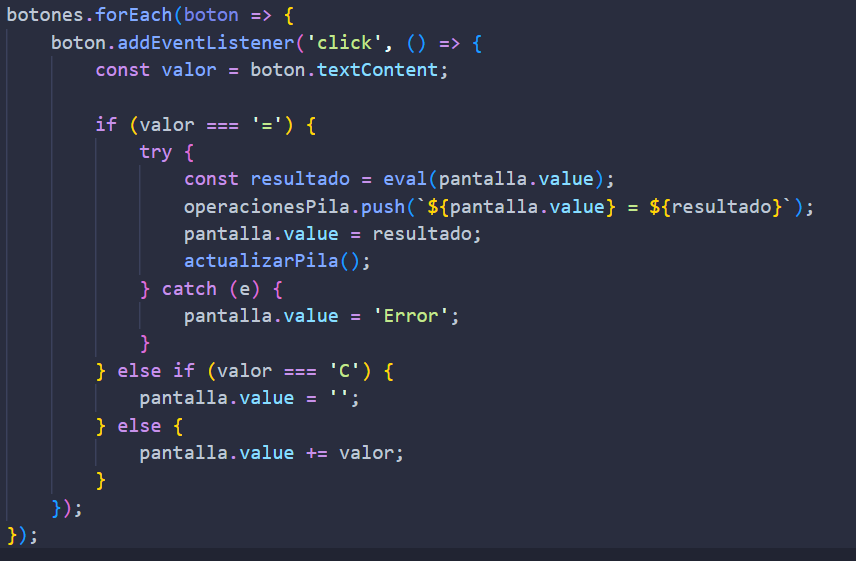
\includegraphics[width=0.8\textwidth,keepaspectratio]                       {img/botonesCal.png}
		             %\includesvg{img/automata.svg}
		              %\label{img:mot2}
		              %\caption{Product backlog.}
    \end{figure}  
\\
\\Función actualizarPila:

\\\textbf{function actualizarPila():} Actualiza la visualización del historial de operaciones.
\\\textbf{pilaOperaciones.innerHTML = '<h3>Historial de Operaciones:</h3>':} Limpia el contenido actual del historial.
\\\textbf{operacionesPila.forEach(operacion =>):} Itera sobre el historial de operaciones.
\\\textbf{const operacionElement = document.createElement('div'):} Crea un nuevo elemento div para cada operación.
\\\textbf{operacionElement.textContent = operacion:} Establece el texto del div con la operación.
\\\textbf{pilaOperaciones.appendChild(operacionElement):} Agrega el div al contenedor del historial.
\begin{figure}[H]
		          \centering
		          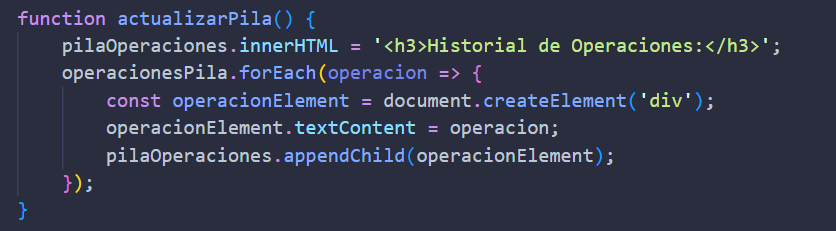
\includegraphics[width=0.8\textwidth,keepaspectratio]                       {img/funcionesCal.png}
		             %\includesvg{img/automata.svg}
		              %\label{img:mot2}
		              %\caption{Product backlog.}
    \end{figure}  
\\
\\Algunas pruebas con su historial de operaciones
\begin{figure}[H]
		          \centering
		          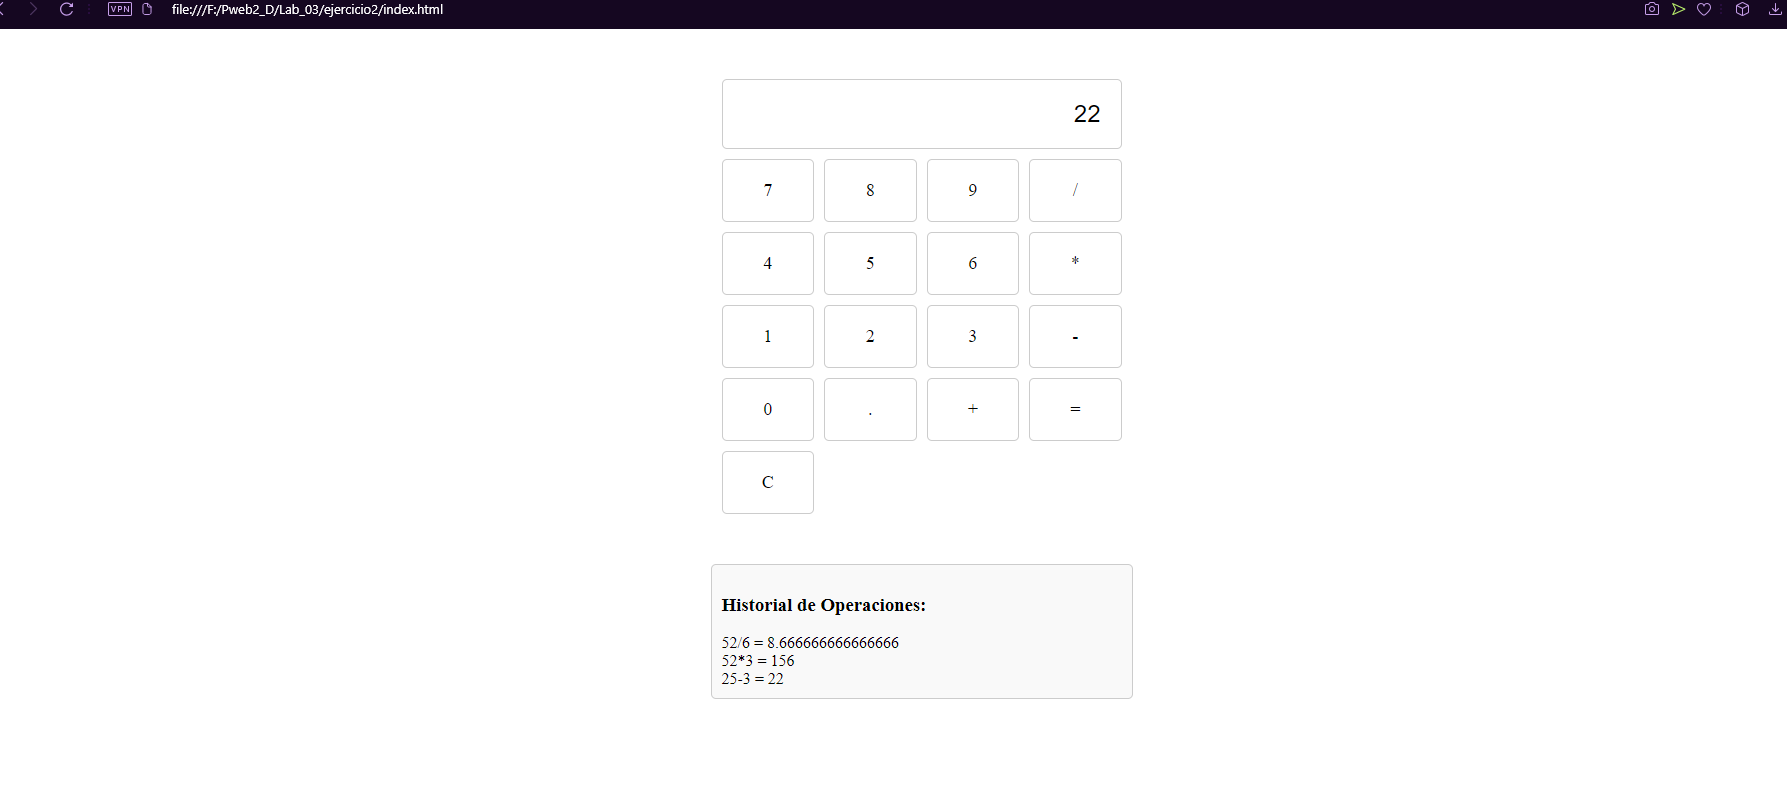
\includegraphics[width=0.8\textwidth,keepaspectratio]                       {img/pruebaCal1.png}
		             %\includesvg{img/automata.svg}
		              %\label{img:mot2}
		              %\caption{Product backlog.}
    \end{figure}  
\\

\begin{figure}[H]
		          \centering
		          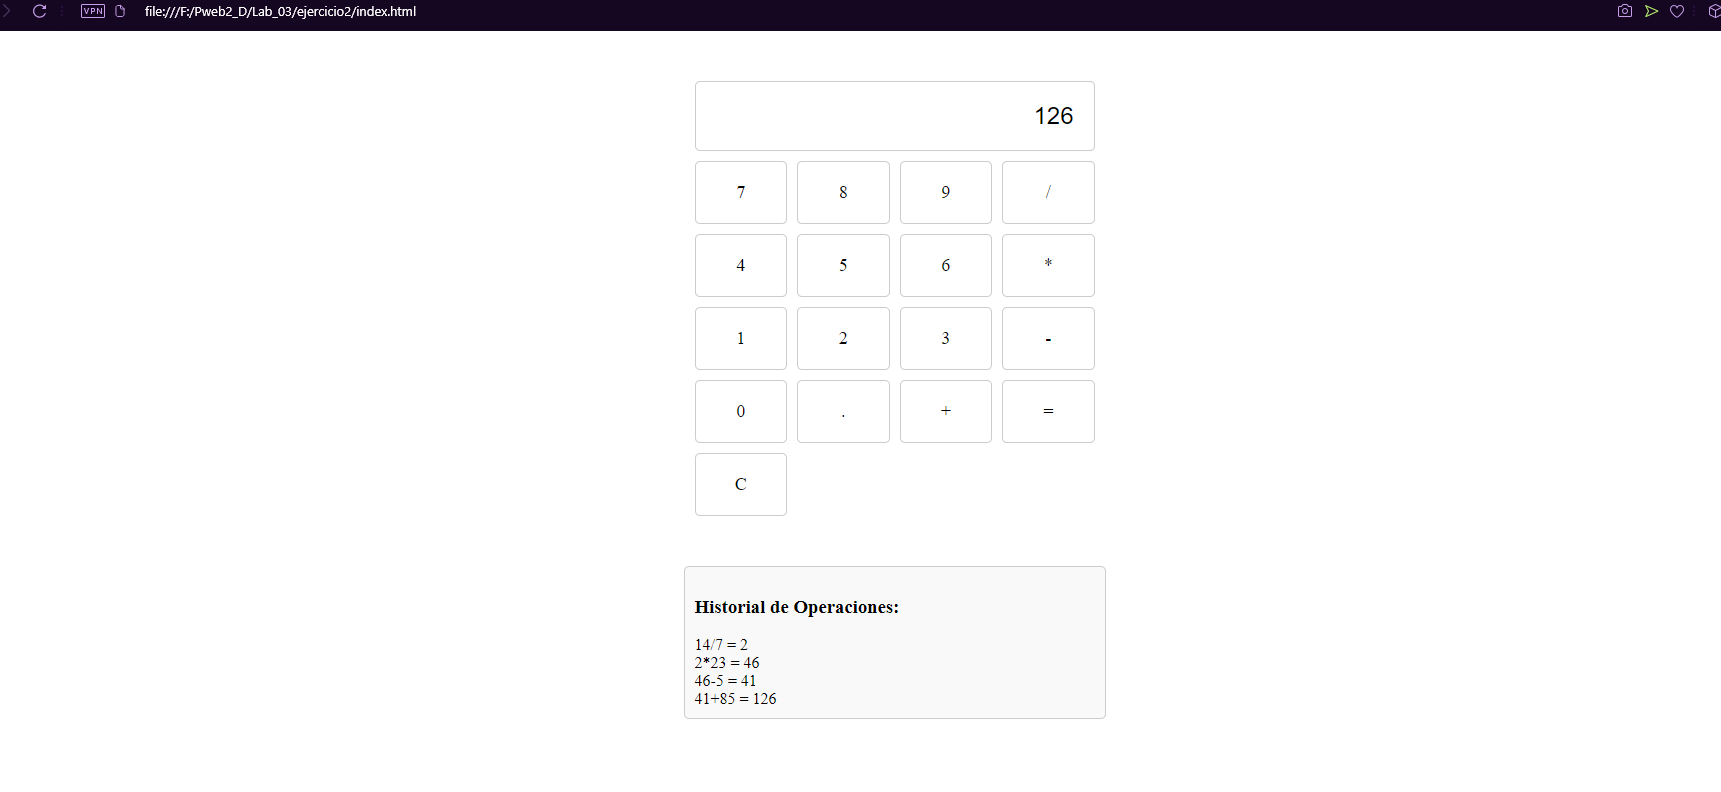
\includegraphics[width=0.8\textwidth,keepaspectratio]                       {img/pruebaCal2.png}
		             %\includesvg{img/automata.svg}
		              %\label{img:mot2}
		              %\caption{Product backlog.}
    \end{figure}  
\\
\subsection{Ejercicio 3}
\\Para este ejercicio igualmente un html basico como en anteriores ejercicios esta vez se usa canvas
\begin{figure}[H]
		          \centering
		          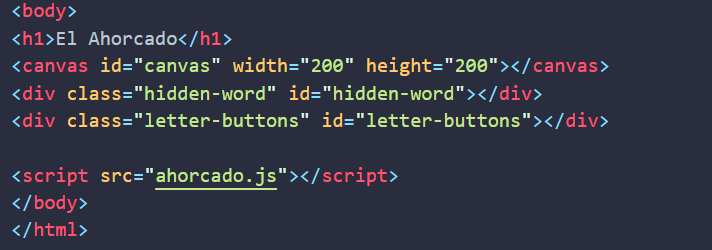
\includegraphics[width=0.8\textwidth,keepaspectratio]                       {img/bodyAh.png}
		             %\includesvg{img/automata.svg}
		              %\label{img:mot2}
		              %\caption{Product backlog.}
    \end{figure}  
\\
\\En la logica tenemos 
\\\textbf{const ctx = canvas.getContext('2d'):} Obtiene el contexto de dibujo en 2D del canvas.
\\\textbf{const hiddenWordElement = document.getElementById('hidden-word'):} Selecciona el elemento que muestra la palabra oculta.
\\\textbf{const letterButtonsElement = document.getElementById('letter-buttons'):} Selecciona el contenedor de botones de letras.
\begin{figure}[H]
		          \centering
		          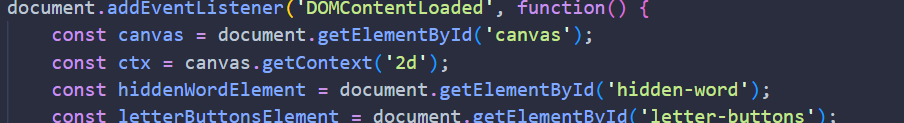
\includegraphics[width=0.8\textwidth,keepaspectratio]                       {img/DOMAh.png}
		             %\includesvg{img/automata.svg}
		              %\label{img:mot2}
		              %\caption{Product backlog.}
    \end{figure}  
\\
\begin{itemize}
    \item \\let palabraSeleccionada = palabras[Math.floor(Math.random() * palabras.length)]: Selecciona una palabra aleatoria del arreglo de palabras.
    \item \\let palabraOculta = Array(palabraSeleccionada.length).fill('_'): Inicializa la palabra oculta con guiones bajos, uno por cada letra de la palabra seleccionada.
    \item \\let intentos = 0: Inicializa el número de intentos a cero.
    \item \\const maxIntentos = 6 : Define el número máximo de intentos permitidos.
\end{itemize}
\\
\\
\begin{figure}[H]
		          \centering
		          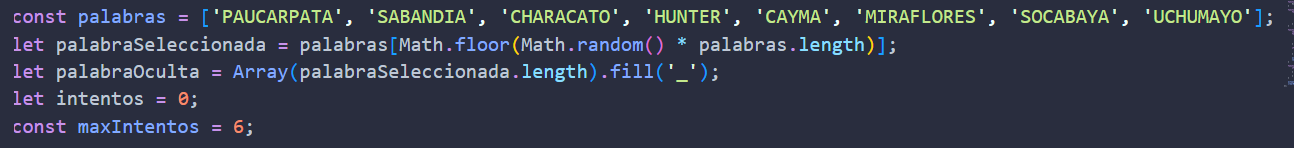
\includegraphics[width=0.8\textwidth,keepaspectratio]                       {img/varAh.png}
		             %\includesvg{img/automata.svg}
		              %\label{img:mot2}
		              %\caption{Product backlog.}
\end{figure}  
\\Función dibujarAhorcado(intentos)
\\Dibuja el progreso del ahorcado en el canvas basado en el número de intentos.
\\Base y poste vertical
\begin{figure}[H]
		          \centering
		          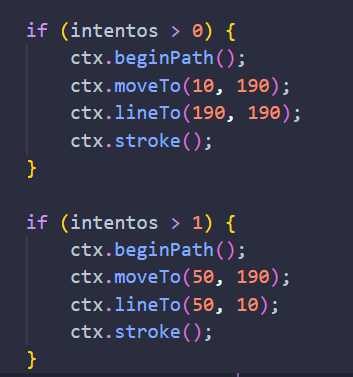
\includegraphics[width=0.8\textwidth,keepaspectratio]                       {img/baseAh.png}
		             %\includesvg{img/automata.svg}
		              %\label{img:mot2}
		              %\caption{Product backlog.}
    \end{figure}  
\\
\\Poste horizontal cuerda y cabeza etc
\begin{figure}[H]
		          \centering
		          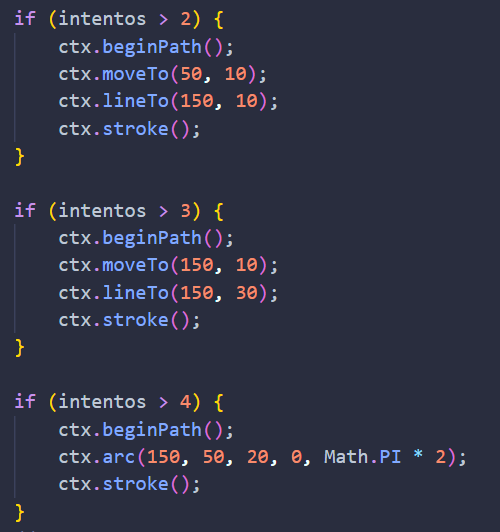
\includegraphics[width=0.8\textwidth,keepaspectratio]                       {img/horAh.png}
		             %\includesvg{img/automata.svg}
		              %\label{img:mot2}
		              %\caption{Product backlog.}
    \end{figure}  
\\
\\Función actualizarPalabraOculta
\\Esta función actualiza la visualización de la palabra oculta en el DOM.
\begin{figure}[H]
		          \centering
		          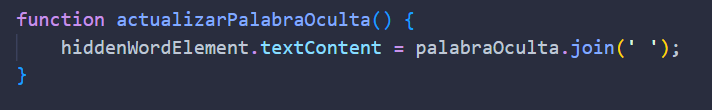
\includegraphics[width=0.8\textwidth,keepaspectratio]                       {img/actAh.png}
		             %\includesvg{img/automata.svg}
		              %\label{img:mot2}
		              %\caption{Product backlog.}
    \end{figure}  
\\
\\Función crearBotonesLetras
\\Esta función crea botones para cada letra del albecedario y les asigna un evento click.
\begin{figure}[H]
		          \centering
		          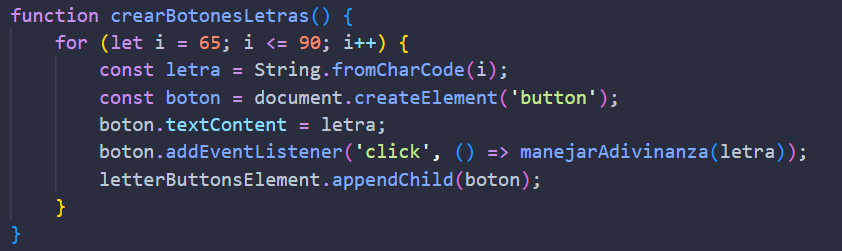
\includegraphics[width=0.8\textwidth,keepaspectratio]                       {img/creAh.png}
		             %\includesvg{img/automata.svg}
		              %\label{img:mot2}
		              %\caption{Product backlog.}
    \end{figure}  
\\

\\Función manejarAdivinanza
\\Maneja el evento cuando se adivina una letra, actualizando la palabra oculta y dibujando el ahorcado si la letra no está en la palabra.
\begin{figure}[H]
		          \centering
		          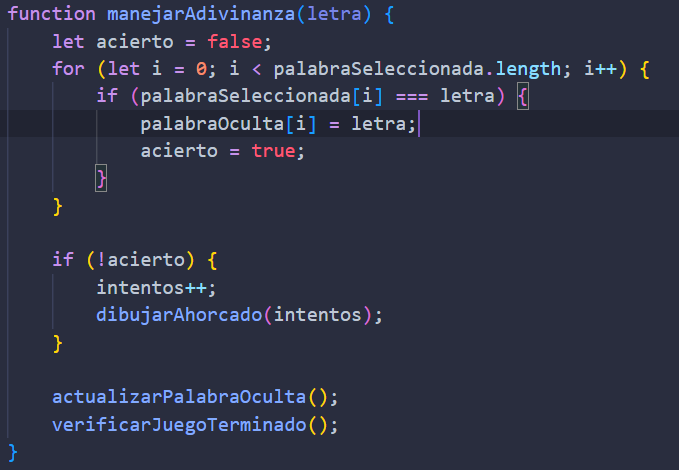
\includegraphics[width=0.8\textwidth,keepaspectratio]                       {img/maneAh.png}
		             %\includesvg{img/automata.svg}
		              %\label{img:mot2}
		              %\caption{Product backlog.}
    \end{figure}  
\\

\\Función verificarJuegoTerminado
\\Verifica si el juego ha terminado, ya sea por adivinar toda la palabra o por alcanzar el número máximo de intentos.
\begin{figure}[H]
		          \centering
		          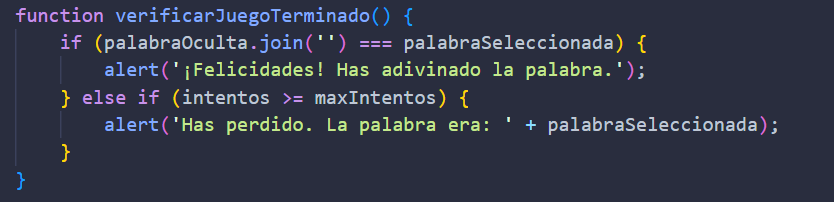
\includegraphics[width=0.8\textwidth,keepaspectratio]                       {img/veriAh.png}
		             %\includesvg{img/automata.svg}
		              %\label{img:mot2}
		              %\caption{Product backlog.}
    \end{figure}  
\\
\\Finalmente inicializan la visualización de la palabra oculta y crean los botones de letras cuando se carga la página.
\begin{figure}[H]
		          \centering
		          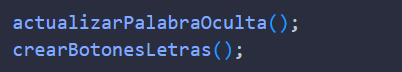
\includegraphics[width=0.8\textwidth,keepaspectratio]                       {img/lanzAh.png}
		             %\includesvg{img/automata.svg}
		              %\label{img:mot2}
		              %\caption{Product backlog.}
    \end{figure}  
\\

\\teclado ofuzcado
\begin{figure}[H]
		          \centering
		          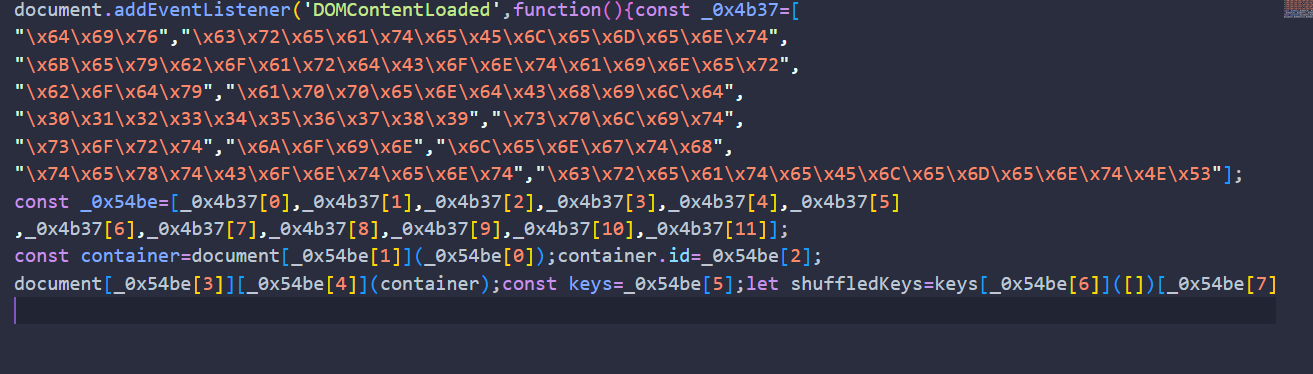
\includegraphics[width=0.8\textwidth,keepaspectratio]                       {img/ofuzcar.png}
		             %\includesvg{img/automata.svg}
		              %\label{img:mot2}
		              %\caption{Product backlog.}
    \end{figure}  
\\
\end{document}